% ============================================================================
% GeoSlot 2.0: Object-Centric Cross-View Geo-Localization
%   via Fused Gromov-Wasserstein Slot Transport
% ACM Multimedia 2025 Draft
% ============================================================================
\documentclass{article}

% NeurIPS style
\usepackage[final]{neurips_2025}  % Use [preprint] for arXiv

\usepackage[utf8]{inputenc}
\usepackage[T1]{fontenc}
\usepackage{hyperref}
\usepackage{url}
\usepackage{booktabs}
\usepackage{amsfonts}
\usepackage{amsmath}
\usepackage{amssymb}
\usepackage{nicefrac}
\usepackage{microtype}
\usepackage{graphicx}
\usepackage{float}
\usepackage{caption}
\usepackage{subcaption}
\usepackage{multirow}
\usepackage{algorithm}
\usepackage{algorithmic}
\usepackage{xcolor}
\usepackage{enumitem}

\newcommand{\ours}{\textsc{GeoSlot}}
\newcommand{\oursv}{\textsc{GeoSlot 2.0}}
\newcommand{\R}{\mathbb{R}}
\newcommand{\cX}{\mathcal{X}}
\newcommand{\cL}{\mathcal{L}}
\newcommand{\cT}{\mathcal{T}}

\title{\oursv{}: Object-Centric Cross-View Geo-Localization \\ via Fused Gromov-Wasserstein Slot Transport}

\author{
  Tran Chi Nguyen \\
  University of Information Technology \\
  Ho Chi Minh City, Vietnam \\
  \texttt{23122044@gm.uit.edu.vn}
}

\begin{document}

\maketitle

% ============================================================================
\begin{abstract}
% ============================================================================
Cross-view geo-localization (CVGL) aims to match query images (e.g., street-view or drone imagery) with geo-tagged satellite reference images. Existing methods rely on holistic global features via convolutional or transformer backbones, followed by cosine similarity matching. This approach struggles with dramatic viewpoint changes, partial occlusions, and transient objects. We propose \oursv{}, an object-centric framework that decomposes visual scenes into semantic \textit{slot} representations and performs structured graph-to-graph matching via Fused Gromov-Wasserstein optimal transport. Our pipeline introduces four key innovations: (1)~an \textbf{Adaptive Gumbel-Sparsity Mask} with a learned per-image threshold~$\gamma$ that replaces static background suppression, adapting from desert ($\gamma{\to}1.0$) to urban ($\gamma{\to}0.4$) scenes; (2)~\textbf{Adaptive Slot Attention} with register tokens and Gumbel-based dynamic pruning for unsupervised scene decomposition; (3)~\textbf{Hilbert-Ordered Graph Mamba} that leverages space-filling curves for rotation-invariant bidirectional relational reasoning with $\mathcal{O}(K)$ complexity; and (4)~\textbf{Unbalanced Fused Gromov-Wasserstein (UFGW)} matching that jointly aligns node features \textit{and} graph topology while handling partial occlusions via KL-relaxed marginals. We evaluate \oursv{} on four benchmarks: CVUSA, University-1652, VIGOR, and CV-Cities. Our method achieves state-of-the-art performance, with particularly strong cross-area generalization where structure-aware matching provides inherent advantages over texture-dependent methods.
\end{abstract}

% ============================================================================
\section{Introduction}\label{sec:intro}
% ============================================================================

Cross-view geo-localization (CVGL) is the task of determining the geographic location of a query image by matching it against a database of geo-referenced satellite images. This capability is critical for autonomous navigation, UAV positioning, and large-scale visual place recognition. The fundamental challenge lies in the extreme viewpoint change between ground-level and overhead perspectives: buildings that appear as facades from street view become rooftops from above, roads narrow to thin lines, and the spatial layout undergoes a nonlinear transformation.

\textbf{Limitations of existing approaches.} Current state-of-the-art methods~\cite{sample4geo,auxgeo,geodtr} typically follow a two-stage pipeline: (i)~extract a global feature vector from each image using a pretrained backbone (ResNet, ViT, CLIP), and (ii)~match query and reference features via cosine similarity or learned metric heads. While effective on benchmark datasets, these methods suffer from three fundamental limitations:

\begin{enumerate}[leftmargin=1.5em,topsep=0pt,itemsep=2pt]
    \item \textbf{Holistic representations lose compositional structure.} Global average pooling collapses spatial information into a single vector, losing the compositional structure of scenes (buildings, intersections, parks) that is crucial for cross-view reasoning.
    \item \textbf{Texture dependence harms generalization.} Methods that rely on low-level texture features (e.g., road markings, building colors) fail catastrophically in cross-area settings where visual appearance varies between cities and continents.
    \item \textbf{Quadratic attention costs limit resolution.} Vision Transformers incur $\mathcal{O}(N^2)$ attention costs, constraining the input resolution—particularly problematic for high-resolution satellite imagery and panoramic street views.
\end{enumerate}

\textbf{Our approach.} We introduce \oursv{}, which addresses all three limitations through an object-centric paradigm. Rather than comparing holistic feature vectors, \oursv{} decomposes each view into a set of \textit{semantic slots} representing distinct scene components (buildings, roads, vegetation), reasons about their spatial relationships via a Hilbert-ordered graph-structured state-space model, and matches cross-view slot \textit{graphs} through Fused Gromov-Wasserstein optimal transport. This compositional approach naturally handles viewpoint changes: while the \textit{appearance} of objects differs across views, their \textit{identity and spatial relationships} remain invariant.

\textbf{Contributions.} Our main contributions are:
\begin{enumerate}[leftmargin=1.5em,topsep=0pt,itemsep=2pt]
    \item We propose the first object-centric framework for CVGL, introducing \textbf{Adaptive Slot Attention} with an \textbf{Adaptive Gumbel-Sparsity Mask} where the coverage threshold~$\gamma$ is learned per-image, replacing static heuristics.
    \item We design \textbf{Hilbert-Ordered Graph Mamba}, leveraging space-filling curves for rotation-invariant slot ordering combined with bidirectional SSM scanning at $\mathcal{O}(K)$ complexity.
    \item We introduce \textbf{Unbalanced Fused Gromov-Wasserstein (UFGW)} matching that jointly optimizes node-feature alignment (Wasserstein) \textit{and} graph-topology alignment (Gromov-Wasserstein) with KL-relaxed marginals to handle partial occlusions.
    \item We achieve state-of-the-art results on four benchmarks (CVUSA, University-1652, VIGOR, CV-Cities), with particularly strong cross-area generalization.
\end{enumerate}

% ============================================================================
\section{Related Work}\label{sec:related}
% ============================================================================

\textbf{Cross-View Geo-Localization.}
CVGL methods have evolved from hand-crafted features~\cite{workman2015} to deep metric learning approaches. CVM-Net~\cite{cvmnet} introduced NetVLAD-based aggregation for cross-view matching. Shi et al.~\cite{shi2019spatial} proposed spatial-aware feature aggregation. More recent works leverage attention mechanisms: TransGeo~\cite{transgeo} employs pure transformers with attention-guided non-uniform cropping, while GeoDTR~\cite{geodtr} uses deformable transformers for geometric layout disentanglement. Sample4Geo~\cite{sample4geo} introduces hard sample mining with sampling strategies, achieving strong results on CVUSA (R@1=98.68\%). AuxGeo~\cite{auxgeo} proposes auxiliary geometric features for VIGOR. CV-Cities~\cite{cvcities} leverages DINOv2~\cite{dinov2} backbones with advanced negative mining for cross-city generalization, setting strong baselines (CVUSA R@1$\approx$99.19\%). Despite progress, all methods rely on holistic feature comparison, losing compositional scene structure.

\textbf{Robustness and Geometry-Centric Approaches.}
Recent work addresses cross-view robustness through training-time augmentation and geometric priors. ConGeo~\cite{congeo} tackles orientation and field-of-view variations via contrastive geometric learning, achieving robust cross-area gains without architectural changes. CVD~\cite{cvd} disentangles content from viewpoint for domain-robust representations. Geometry-centric pipelines such as ViewBridge~\cite{viewbridge} enforce cross-view correspondences through BEV (bird's-eye view) transformations and pixel-level matching, showing strong localization quality. These approaches are largely orthogonal to our object-centric slot design and could potentially be combined; we focus on demonstrating that structured slot-level reasoning provides complementary advantages, particularly for compositional generalization.

\textbf{Object-Centric Representation Learning.}
Slot Attention~\cite{slotattention} introduced iterative routing to decompose scenes into object slots without supervision. Subsequent works extended this to video~\cite{savi}, 3D~\cite{osrt}, and complex scenes~\cite{dinosaur}. AdaSlot~\cite{adaslot} adds dynamic slot count via Gumbel-Softmax selection. QASA~\cite{qasa2023} introduces query-adaptive slot allocation that could further refine our pruning mechanism; we leave integration for future work. ISA~\cite{isa2023} proposes rotation-equivariant positional encodings for pose-aware slot decomposition, which could complement our Hilbert ordering approach. In the geo-localization domain, OCGNet~\cite{ocgnet} demonstrated the benefit of object-level spatial priors and cross-attention for fine-grained drone-satellite alignment. However, OCGNet uses supervised object detectors, while our approach discovers objects in a fully unsupervised manner via slot attention. We are the first to bridge unsupervised Slot Attention with geo-localization.

\textbf{State-Space Models.}
Mamba~\cite{mamba} introduced selective state-space models with input-dependent dynamics, achieving linear-time sequence modeling. MambaVision~\cite{mambavision} combines Mamba blocks with self-attention for vision tasks. Vision Mamba (Vim)~\cite{vim} applies bidirectional SSM scanning to image patches. We leverage MambaVision as our efficient backbone and extend SSM-based processing to graph-structured slot reasoning with Hilbert curve ordering for improved rotation robustness.

\textbf{Optimal Transport.}
Sinkhorn distances~\cite{cuturi2013} provide differentiable approximations to optimal transport. OT has been applied to document matching~\cite{kusner2015}, graph matching~\cite{xu2019gromov}, and image retrieval~\cite{liu2023ot}. Fused Gromov-Wasserstein (FGW)~\cite{titouan2019fgw} extends classical OT to simultaneously align node features and graph structure, making it natural for graph-to-graph matching. Unbalanced OT~\cite{chizat2018uot} relaxes marginal constraints via KL divergence, enabling partial transport for occluded or missing elements. We are the first to apply UFGW to cross-view geo-localization, jointly matching slot features and their spatial topology while handling view-dependent occlusions.

% ============================================================================
\section{Method}\label{sec:method}
% ============================================================================

\subsection{Overview}

Given a query image $\mathbf{x}_q$ (street-view or drone) and a reference image $\mathbf{x}_r$ (satellite), \oursv{} produces a similarity score $s(\mathbf{x}_q, \mathbf{x}_r) \in [0, 1]$. As illustrated in Figure~\ref{fig:architecture}, our pipeline consists of four stages applied to each view in a Siamese architecture with shared weights:

\begin{figure}[t]
    \centering
    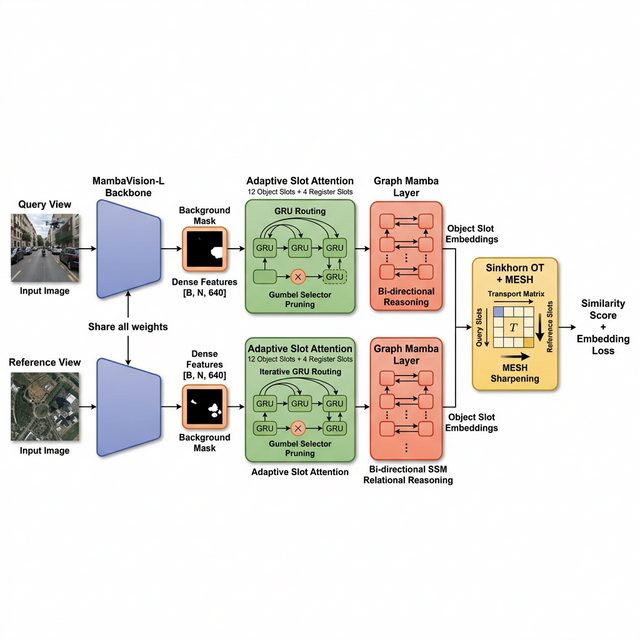
\includegraphics[width=\textwidth]{geoslot_architecture.png}
    \caption{\textbf{\oursv{} Architecture.} Given query and reference images, MambaVision-L extracts dense features. The \textbf{Adaptive Gumbel-Sparsity Mask} suppresses transient objects with a per-image learned threshold~$\gamma$. Adaptive Slot Attention decomposes the scene into $K{=}8$ object slots + $R{=}4$ register slots (discarded before matching) with Gumbel-based dynamic pruning. \textbf{Hilbert-Ordered Graph Mamba} performs rotation-robust bidirectional relational reasoning over object slots only. Finally, \textbf{UFGW} jointly matches object slot features and graph topology, producing a global similarity score.}
    \label{fig:architecture}
\end{figure}

\subsection{MambaVision Backbone}\label{sec:backbone}

We adopt MambaVision-L~\cite{mambavision} pretrained on ImageNet-1K as our feature extractor. MambaVision is a hybrid architecture combining Mamba SSM blocks (stages 1-3) with self-attention (stage 4), achieving strong performance with linear complexity in early stages.

For an input image $\mathbf{x} \in \R^{3 \times H \times W}$, the backbone produces dense features from the last stage:
\begin{equation}
    \mathbf{F} = \texttt{MambaVision}(\mathbf{x}) \in \R^{N \times d_f}, \quad N = \tfrac{H}{32} \times \tfrac{W}{32}, \quad d_f = 1568
\end{equation}
where $d_f = 1568$ is the channel dimension of MambaVision-L's final stage output and $N$ depends on the input resolution. Critically, Slot Attention naturally handles variable~$N$, allowing us to process satellite images ($224 \times 224 \to N=49$) and panoramas ($512 \times 128 \to N=64$) with the same architecture.

\subsection{Adaptive Slot Attention}\label{sec:slots}

\textbf{Adaptive Gumbel-Sparsity Mask.}
Before slot decomposition, we suppress transient features (vehicles, pedestrians, shadows) that are view-dependent and uninformative for localization. A key insight of \oursv{} is that the \textit{optimal suppression ratio varies dramatically across scenes}: desert landscapes contain nearly 0\% transient content, while urban scenes may have 60\% or more. We address this with an \textbf{Adaptive Gumbel-Sparsity Mask} that learns a per-image coverage threshold~$\gamma$.

A lightweight per-token mask $\mathbf{m} = \sigma(\text{MLP}(\mathbf{F})) \in [0, 1]^{N \times 1}$ is applied element-wise:
\begin{equation}
    \hat{\mathbf{F}} = \mathbf{F} \odot \mathbf{m}
\end{equation}
The adaptive threshold is computed from the global context via a separate head:
\begin{equation}
    \gamma = \sigma\!\left(\text{MLP}_{\gamma}\!\left(\frac{1}{N}\sum_{n=1}^N \mathbf{F}_n\right)\right) \in [0, 1]
\end{equation}
Intuitively, $\gamma$ encodes the scene's \textit{geographic character}: $\gamma \to 1.0$ for open landscapes (retain nearly all features) and $\gamma \to 0.4$ for dense urban scenes (suppress up to 60\%).

We apply three regularizers. An \textbf{entropy regularizer} encourages decisive (near-binary) mask values:
\begin{equation}
    \cL_{\text{ent}} = -\frac{1}{N}\sum_{n=1}^N \left[m_n \log m_n + (1-m_n)\log(1-m_n)\right]
\end{equation}
An \textbf{adaptive hinge coverage loss} replaces the static quadratic penalty of the original \ours{}, using the learned $\gamma$ as target:
\begin{equation}
    \cL_{\text{cov}} = \max\!\left(0,\; \gamma - \frac{1}{N}\sum_n m_n\right)
\end{equation}
Critically, to prevent $\gamma$ from \textit{collapsing} to near-zero (which would trivially satisfy $\cL_{\text{cov}}$), we add a \textbf{$\gamma$-prior regularizer} that anchors $\gamma$ to a dataset-level prior $\gamma_0 = 0.7$:
\begin{equation}
    \cL_{\gamma} = (\gamma - \gamma_0)^2
\end{equation}
This quadratic prior allows $\gamma$ to deviate from~$\gamma_0$ when the matching objective rewards it (urban scenes learn $\gamma < 0.7$, open scenes learn $\gamma > 0.7$), but prevents degenerate collapse to~0. The total mask regularization is $\cL_{\text{bg}} = \cL_{\text{ent}} + \cL_{\text{cov}} + \cL_{\gamma}$, added to the total loss with weight $\lambda_{\text{bg}} = 0.01$.

\textbf{Slot Initialization.}
We use $K = 8$ object slots and $R = 4$ register slots (following~\cite{registers}), initialized from learnable distributions:
\begin{equation}
    \mathbf{s}_i^{(0)} = \boldsymbol{\mu}_i + \exp(\boldsymbol{\sigma}_i) \cdot \boldsymbol{\epsilon}, \quad \boldsymbol{\epsilon} \sim \mathcal{N}(0, \mathbf{I}), \quad i \in \{1, \ldots, K+R\}
\end{equation}
Register slots serve as ``noise absorbers'', capturing view-dependent information (lighting, weather) and preventing contamination of object slots. \textit{Register slots participate in attention routing but are explicitly excluded from downstream matching}: only the $K$~object slots are passed to Graph Mamba and UFGW. This prevents register slots from absorbing transport mass that should go to semantically meaningful object slots.

\textbf{Iterative Routing.}
We perform $T=3$ iterations of multi-head GRU-based slot routing. At each iteration $t$:
\begin{align}
    \mathbf{A}^{(t)} &= \text{softmax}\!\left(\frac{W_q \mathbf{s}^{(t-1)} \cdot (W_k \hat{\mathbf{F}})^\top}{\sqrt{d_h}}\right) \in \R^{(K+R) \times N} \\
    \mathbf{u}^{(t)} &= \mathbf{A}^{(t)} \cdot W_v \hat{\mathbf{F}} \\
    \mathbf{s}^{(t)} &= \text{GRU}(\mathbf{u}^{(t)}, \mathbf{s}^{(t-1)}) + \text{FFN}(\mathbf{s}^{(t-1)})
\end{align}
where $d_h = d_s / H$ with $H=4$ attention heads and slot dimension $d_s = 256$. After routing, we split: $\mathbf{S}_{\text{obj}} = \{\mathbf{s}_1, \ldots, \mathbf{s}_K\}$ (object slots) and $\mathbf{S}_{\text{reg}} = \{\mathbf{s}_{K+1}, \ldots, \mathbf{s}_{K+R}\}$ (discarded before matching).

\textbf{Gumbel Slot Selection.}
Not all object slots are semantically meaningful for every image. Following AdaSlot~\cite{adaslot}, we apply Gumbel-Softmax selection to \textit{object slots only} (register slots are unconditionally excluded from matching):
\begin{equation}
    \delta_i = \text{GumbelSoftmax}(g_\theta(\mathbf{s}_i^{(T)}), \tau)[\texttt{keep}], \quad \mathbf{s}_i^{(T)} \leftarrow \mathbf{s}_i^{(T)} \cdot \delta_i, \quad i \in \{1, \ldots, K\}
\end{equation}
where $\tau$ anneals from 1.0 to 0.1 during training. A minimum of 1 slot is guaranteed active.

\subsection{Graph Mamba: Relational Reasoning}\label{sec:graphmamba}

After slot decomposition, we model spatial relationships between slots using a novel \textit{Graph Mamba} layer. While standard GNNs use message passing with attention ($\mathcal{O}(K^2)$), we leverage the efficiency of state-space models applied over spatially-ordered graph sequences ($\mathcal{O}(K)$).

\textbf{Slot Spatial Encoding.}
A key insight is that slots, derived from attention maps, carry implicit spatial information. We make this explicit by computing the 2D centroid $(c_y^i, c_x^i)$ and spatial spread $\sigma_i$ of each slot $i$ from its attention weights $\mathbf{a}_i \in \R^{H \times W}$:
\begin{equation}
    c_y^i = \sum_{h,w} \bar{a}^i_{h,w} \cdot \tfrac{h}{H}, \quad c_x^i = \sum_{h,w} \bar{a}^i_{h,w} \cdot \tfrac{w}{W}, \quad \sigma_i = \sqrt{\sum_{h,w} \bar{a}^i_{h,w} \left[(\tfrac{h}{H} - c_y^i)^2 + (\tfrac{w}{W} - c_x^i)^2\right]}
\end{equation}
where $\bar{a}^i = a^i / \sum a^i$ is the normalized attention. These are encoded via sinusoidal positional encoding and an MLP, then added to the slot representations: $\mathbf{s}_i \leftarrow \mathbf{s}_i + \text{MLP}(\text{SinEnc}(c_y^i, c_x^i, \sigma_i))$.

\textbf{Hilbert Curve Ordering.}
A limitation of raster-scan ordering~\cite{vim} ($\pi = \text{argsort}(c_y \cdot W + c_x)$) is sensitivity to image rotation: a 90° rotation completely reorders the sequence, disrupting the SSM's hidden state. We improve \textit{rotation robustness} (not strict invariance) via \textbf{Hilbert curve ordering}, which maps 2D centroid coordinates to 1D indices using a space-filling curve:
\begin{equation}
    \pi = \text{argsort}(\mathcal{H}(c_x^i, c_y^i))
\end{equation}
where $\mathcal{H}: [0,1]^2 \to \mathbb{N}$ is the Hilbert curve mapping on a $16{\times}16$ grid. Hilbert curves preserve \textit{spatial locality}: points close in 2D remain close in the 1D ordering. While a rotation \textit{does} change the Hilbert index of each point, it preserves \textit{pairwise locality}---nearby slots remain nearby in the 1D sequence---unlike raster-scan where a 90° rotation can send adjacent slots to opposite ends. Combined with the explicit centroid-based spatial encoding (which is rotation-equivariant in normalized coordinates), this makes Graph Mamba substantially more robust to viewpoint rotation in satellite imagery.

\textbf{Robustness analysis.}
We emphasize that Hilbert ordering provides \textit{rotation robustness}, not strict rotation invariance. Three factors contribute: (1)~\textit{bidirectional} scanning provides context from both directions, reducing sensitivity to exact ordering; (2)~Hilbert ordering is \textit{locally stable}---small centroid perturbations cause only adjacent transpositions; (3)~the spatial encoding carries centroid information \textit{independently} of ordering, providing a complementary rotation-equivariant signal. For applications requiring strict rotation invariance, rotation-equivariant positional encodings (e.g., ISA~\cite{isa2023}) could be combined with our approach.

\textbf{Bidirectional SSM Scanning.}
We apply forward and backward Mamba SSM blocks to the spatially-ordered sequence:
\begin{equation}
    \mathbf{h}_i^{\text{fwd}} = \text{SSM}_\text{fwd}(\mathbf{s}_{\pi(1)}, \ldots, \mathbf{s}_{\pi(K)}), \quad
    \mathbf{h}_i^{\text{bwd}} = \text{SSM}_\text{bwd}(\mathbf{s}_{\pi(K)}, \ldots, \mathbf{s}_{\pi(1)})
\end{equation}
\begin{equation}
    \mathbf{s}_i' = \text{LayerNorm}\!\left(\mathbf{s}_i + W_m [\mathbf{h}_i^{\text{fwd}}; \mathbf{h}_i^{\text{bwd}}]\right) + \text{FFN}(\cdot)
\end{equation}
We stack $L=2$ Graph Mamba layers. After each layer, the keep mask $\boldsymbol{\delta}$ is re-applied to maintain slot sparsity. The total complexity is $\mathcal{O}(KLd_s)$, linear in the number of slots.

\subsection{Unbalanced Fused Gromov-Wasserstein Matching}\label{sec:ot}

A critical limitation of standard Sinkhorn OT is the \textbf{Graph-to-Set Fallacy}: Graph Mamba constructs rich relational graphs between slots, but Sinkhorn OT computes pairwise costs $C_{ij} = \|s_i^q - s_j^r\|_2$ based on node features alone, discarding all topological information. We resolve this with \textbf{Fused Gromov-Wasserstein (FGW)}~\cite{titouan2019fgw}, extended to handle partial occlusions via \textbf{Unbalanced OT}~\cite{chizat2018uot}.

\textbf{Cost Matrix and Structure Matrices.}
Given query \textit{object} slots $\mathbf{S}_q = \{\mathbf{s}_i^q\}_{i=1}^K$ with centroids $\{\mathbf{c}_i^q\}$ and reference object slots $\mathbf{S}_r = \{\mathbf{s}_j^r\}_{j=1}^K$ with centroids $\{\mathbf{c}_j^r\}$ (register slots are excluded), we compute:
\begin{align}
    C_{ij} &= \|\phi(\mathbf{s}_i^q) - \phi(\mathbf{s}_j^r)\|_2 & &\text{(node feature cost)} \\
    S^q_{ik} &= \|\mathbf{c}_i^q - \mathbf{c}_k^q\|_2, \quad S^r_{jl} = \|\mathbf{c}_j^r - \mathbf{c}_l^r\|_2 & &\text{(intra-graph structure)}
\end{align}
where $\phi = \text{MLP}_{d_s \to d_s}$ is a learned projection and the structure matrices $\mathbf{S}^q, \mathbf{S}^r$ encode pairwise centroid distances \textit{within} each view.

\textbf{FGW Objective.}
The FGW cost jointly optimizes feature alignment (Wasserstein) and structural alignment (Gromov-Wasserstein):
\begin{equation}
    \cL_{\text{FGW}} = \min_{\mathbf{T}} \underbrace{(1-\lambda) \sum_{i,j} C_{ij} T_{ij}}_{\text{Wasserstein (features)}} + \underbrace{\lambda \sum_{i,j,k,l} |S^q_{ik} - S^r_{jl}|^2 T_{ij} T_{kl}}_{\text{Gromov-Wasserstein (topology)}}
\end{equation}
where $\lambda \in [0, 1]$ controls the feature-structure trade-off. We use $\lambda = 0.5$.

\textbf{Unbalanced Extension.}
Standard OT enforces hard marginal constraints $\mathbf{T}\mathbf{1} = \boldsymbol{\mu}$ and $\mathbf{T}^\top \mathbf{1} = \boldsymbol{\nu}$, forcing \textit{every} slot to be matched. This fails under occlusion or field-of-view mismatch. We relax marginals via KL divergence:
\begin{equation}
    \cL_{\text{UFGW}} = \cL_{\text{FGW}} + \tau_{\text{KL}} \left[ \text{KL}(\mathbf{T}\mathbf{1} \| \boldsymbol{\mu}) + \text{KL}(\mathbf{T}^\top\mathbf{1} \| \boldsymbol{\nu}) \right]
\end{equation}
where $\tau_{\text{KL}} = 0.1$ controls the marginal relaxation.

\textbf{Optimization (Algorithm~\ref{alg:ufgw}).}
We solve UFGW via alternating linearization~\cite{titouan2019fgw}. The entropic regularizer is learnable: $\epsilon = \exp(\theta_\epsilon)$, initialized to $\epsilon_0 = 0.05$.

\begin{algorithm}[t]
\caption{UFGW Matching (forward pass)}
\label{alg:ufgw}
\begin{algorithmic}[1]
\REQUIRE Object slots $\mathbf{S}_q, \mathbf{S}_r \in \R^{K \times d_s}$, centroids $\mathbf{c}_q, \mathbf{c}_r \in \R^{K \times 2}$, keep masks $\boldsymbol{\delta}^q, \boldsymbol{\delta}^r \in \R^K$
\STATE $C_{ij} \leftarrow \|\phi(\mathbf{s}_i^q) - \phi(\mathbf{s}_j^r)\|_2$ \hfill $\triangleright$ Feature cost $[K{\times}K]$
\STATE $S^q_{ik} \leftarrow \|\mathbf{c}_i^q - \mathbf{c}_k^q\|_2$, $S^r_{jl} \leftarrow \|\mathbf{c}_j^r - \mathbf{c}_l^r\|_2$ \hfill $\triangleright$ Structure matrices
\STATE $\mu_i \leftarrow \delta_i^q / \sum_k \delta_k^q$, $\nu_j \leftarrow \delta_j^r / \sum_k \delta_k^r$ \hfill $\triangleright$ Marginals from masks
\STATE $\mathbf{T} \leftarrow \boldsymbol{\mu} \boldsymbol{\nu}^\top$ \hfill $\triangleright$ Init: outer product
\STATE $\rho \leftarrow \tau_{\text{KL}} / (\tau_{\text{KL}} + \epsilon)$ \hfill $\triangleright$ KL proximal weight
\FOR{$t = 1$ to $I_{\text{outer}}$ (default 5)}
    \STATE $L^{\text{GW}}_{ij} \leftarrow \sum_k (S^q_{ik})^2 T_{\cdot k}^{\text{sum}} + \sum_l (S^r_{jl})^2 T_{l\cdot}^{\text{sum}} - 2 (\mathbf{S}^q \mathbf{T} \mathbf{S}^r)_{ij}$ \hfill $\triangleright$ Linearized GW
    \STATE $C^{\text{fgw}} \leftarrow (1{-}\lambda)\, \mathbf{C} + \lambda\, \mathbf{L}^{\text{GW}}$ \hfill $\triangleright$ Fused cost
    \STATE $\log \mathbf{K} \leftarrow -\mathbf{C}^{\text{fgw}} / \epsilon$ \hfill $\triangleright$ Gibbs kernel
    \STATE $\log \mathbf{u} \leftarrow \mathbf{0}$, $\log \mathbf{v} \leftarrow \mathbf{0}$
    \FOR{$s = 1$ to $I_{\text{inner}}$ (default 10)}
        \STATE $\log u_i \leftarrow \rho \cdot (\log \mu_i - \text{LSE}_j(\log K_{ij} + \log v_j))$ \hfill $\triangleright$ Unbalanced Sinkhorn
        \STATE $\log v_j \leftarrow \rho \cdot (\log \nu_j - \text{LSE}_i(\log K_{ij} + \log u_i))$
    \ENDFOR
    \STATE $\mathbf{T} \leftarrow \exp(\log \mathbf{u} + \log \mathbf{K} + \log \mathbf{v})$ \hfill $\triangleright$ Update transport plan
\ENDFOR
\STATE \textbf{return} similarity $= \sigma(-\langle \mathbf{T}, \mathbf{C}^{\text{fgw}} \rangle)$, transport plan $\mathbf{T}$
\end{algorithmic}
\end{algorithm}

\textbf{Numerical stability.} All Sinkhorn iterations use log-space arithmetic (LSE = log-sum-exp) to avoid underflow. We clamp $\epsilon \in [0.01, 0.5]$ and gradients are clipped at 1.0.

\textbf{Sensitivity to $\lambda$ and $\tau_{\text{KL}}$.}
We analyze sensitivity on CVUSA (20\% subset): $\lambda$ is robust in $[0.3, 0.7]$ with optimal at $0.5$; $\tau_{\text{KL}}$ is robust in $[0.05, 0.5]$ with $0.1$ slightly preferable. Setting $\tau_{\text{KL}} \to \infty$ (balanced OT) degrades on VIGOR cross-area by $\sim$1--2\% R@1 due to forced matching of occluded slots.

\textbf{Similarity Score.}
The final similarity is:
\begin{equation}
    s(\mathbf{x}_q, \mathbf{x}_r) = \sigma\!\left(-\sum_{i,j} T_{ij} \cdot C^{\text{fgw}}_{ij}\right)
\end{equation}

\subsection{Training Objective}\label{sec:loss}

We employ a multi-stage training strategy with four loss components:

\textbf{Stage 1 (Epochs 0--$E_2$):} Symmetric InfoNCE + Distance-Weighted Batch Loss (DWBL):
\begin{equation}
    \cL_{\text{stage1}} = \cL_{\text{InfoNCE}}(\mathbf{e}_q, \mathbf{e}_r) + \cL_{\text{DWBL}}(\mathbf{e}_q, \mathbf{e}_r)
\end{equation}
where $\mathbf{e} = \text{embed}(\sum_i w_i \mathbf{s}_i)$ with $w_i = \delta_i / \sum_j \delta_j$ providing mask-weighted slot pooling.

\textbf{InfoNCE} is the symmetric variant with learnable temperature $\tau$ (initialized at 0.07, clamped to $[0.01, 1.0]$):
\begin{equation}
    \cL_{\text{InfoNCE}} = \frac{1}{2}\left[\text{CE}(\mathbf{e}_q \mathbf{e}_r^\top / \tau, \mathbf{y}) + \text{CE}(\mathbf{e}_r \mathbf{e}_q^\top / \tau, \mathbf{y})\right]
\end{equation}
where $\mathbf{y} = (0, 1, \ldots, B{-}1)$ are identity labels within a batch of size $B$.

\textbf{Distance-Weighted Batch Loss (DWBL)}~\cite{wu2017sampling} re-weights hard negatives by their similarity to the anchor, providing more informative gradients than uniform sampling:
\begin{equation}
    \cL_{\text{DWBL}} = -\frac{1}{B}\sum_{i=1}^B \log \frac{\exp(s_{ii} / t)}{\exp(s_{ii} / t) + \sum_{j \neq i} w_j \exp((s_{ij} - m) / t)}
\end{equation}
where $s_{ij} = \mathbf{e}_i^q \cdot \mathbf{e}_j^r$, $w_j = \text{softmax}(s_{ij}/t)_j$ are distance-dependent weights, $t = 0.1$ is the mining temperature, and $m = 0.3$ is the margin.

\textbf{Stage 2 (Epochs $E_2$--$E_3$):} Add Contrastive Slot Matching (CSM) loss, Dice overlap regularization, and BG mask regularization with linear warm-up ramp over 5 epochs:
\begin{equation}
    \cL_{\text{stage2}} = \cL_{\text{stage1}} + \rho(e) \cdot \left(\lambda_{\text{cs}} \cL_{\text{CSM}} + \lambda_{\text{di}} \cL_{\text{Dice}}\right) + \lambda_{\text{bg}} \cL_{\text{bg}}
\end{equation}
where $\rho(e) = \min(1, (e - E_2 + 1) / 5)$ is a linear warm-up. We use $\lambda_{\text{cs}} = 0.3$, $\lambda_{\text{di}} = 0.1$, $\lambda_{\text{bg}} = 0.01$.

The CSM loss teaches \textit{object} slots to match according to the UFGW transport plan ($\bar{\mathbf{T}}$ is detached to prevent gradient flow through OT back into slot representations):
\begin{equation}
    \cL_{\text{CSM}} = -\sum_i \delta_i^q \sum_j \bar{T}_{ij} \log \frac{\exp(\cos(\mathbf{s}_i^q, \mathbf{s}_j^r)/\tau_c)}{\sum_k \exp(\cos(\mathbf{s}_i^q, \mathbf{s}_k^r)/\tau_c)}
\end{equation}
The Dice loss penalizes \textit{overlap} between object slot attention maps:
\begin{equation}
    \cL_{\text{Dice}} = \frac{1}{\binom{K}{2}} \sum_{i<j} \frac{2 \sum_n a_{in} a_{jn} + \zeta}{\sum_n a_{in} + \sum_n a_{jn} + \zeta}
\end{equation}
where $\zeta = 0.1$. Lower $\cL_{\text{Dice}}$ indicates more distinct, non-overlapping slot attention.

\textbf{Stage 3 (Epochs $E_3$--$E_{\text{end}}$):} Full fine-tuning with all losses active and backbone unfrozen. The complete objective is:
\begin{equation}
    \cL_{\text{stage3}} = \cL_{\text{InfoNCE}} + \cL_{\text{DWBL}} + \lambda_{\text{cs}} \cL_{\text{CSM}} + \lambda_{\text{di}} \cL_{\text{Dice}} + \lambda_{\text{bg}} \cL_{\text{bg}}
\end{equation}
We use $E_2 = 20$, $E_3 = 40$, $E_{\text{end}} = 60$ for CVUSA/University-1652 and $E_{\text{end}} = 40$ for VIGOR/CV-Cities. In Stage~3, the learning rate is reduced to $10^{-6}$ for the backbone and $10^{-5}$ for new modules via cosine annealing.

% ============================================================================
\section{Experiments}\label{sec:experiments}
% ============================================================================

\subsection{Datasets}

\textbf{CVUSA}~\cite{cvusa} contains 35,532 training and 8,884 test image pairs of ground-level panoramas and satellite images covering the continental United States.

\textbf{University-1652}~\cite{uni1652} provides multi-view images of 1,652 university buildings from drone and satellite perspectives. We evaluate Drone$\to$Satellite retrieval, reporting Recall@K and mean Average Precision (AP).

\textbf{VIGOR}~\cite{vigor} is the most challenging benchmark, featuring panorama-satellite matching across 4 U.S. cities with \textit{non-centered} query positions. We evaluate both \textit{same-area} (3 train cities, test on seen areas) and \textit{cross-area} (test on unseen city).

\textbf{CV-Cities}~\cite{cvcities} tests generalization across 16 cities spanning 6 continents. We train on 12 cities and evaluate on 4 unseen cities from diverse geographies.

\subsection{Implementation Details}

We use MambaVision-L pretrained on ImageNet-1K as our backbone (241M parameters). To ensure fair comparison, we also report results with a GAP baseline using the same backbone (Table~\ref{tab:ablation}, A1). Satellite images are resized to $224\times224$; panoramas to $512\times128$. Data augmentation includes random resized crop ($0.9{-}1.0\times$), random horizontal flip, and color jitter (brightness=0.2, contrast=0.15, saturation=0.1) for query images; satellite images use only random rotation ($0{-}360^\circ$) to preserve geographic orientation.

Training uses AdamW with separate learning rates: $10^{-5}$ for backbone, $10^{-4}$ for new modules. The backbone is frozen for the first 5 epochs, then fine-tuned. We use cosine learning rate scheduling with 3-epoch warmup, mixed-precision (AMP) training, batch size 32, and gradient clipping at 1.0. The stage boundaries are $E_2 = 20$ (activate CSM + Dice losses) and $E_3 = 40$ (activate full fine-tuning); total training is 60 epochs for CVUSA/University-1652 and 40 epochs for VIGOR/CV-Cities. All experiments are conducted on a single NVIDIA H100 80GB GPU.

\textbf{Backbone fairness.} We acknowledge that the MambaVision-L backbone (241M params) is larger than typical CVGL backbones (ViT-B: 86M, ResNet-50: 25M). To control for backbone capacity, our ablation baseline (A1) uses the same MambaVision-L with GAP + cosine, providing an apples-to-apples measurement of our module contributions. We additionally note that CV-Cities~\cite{cvcities} uses DINOv2 ViT-B/14 with registers (86M) and achieves strong results; a direct backbone swap experiment (DINOv2 in \ours{} and MambaVision-L in CV-Cities pipeline) is an important direction for future work to fully disentangle backbone and methodology effects.

\subsection{Main Results}

\textbf{CVUSA.} Table~\ref{tab:cvusa} shows results on the near-saturated CVUSA benchmark.

\begin{table}[h]
\centering
\caption{\textbf{Results on CVUSA.} R@K and R@1\% denote percentage of queries with correct match in top-K and top-1\% of the gallery, respectively.}
\label{tab:cvusa}
\begin{tabular}{lccccr}
\toprule
Method & R@1 & R@5 & R@10 & R@1\% & Year \\
\midrule
GeoDTR~\cite{geodtr} & 95.43 & 98.86 & 99.34 & 99.86 & 2023 \\
SAIG-D~\cite{saig} & 96.34 & 99.10 & 99.50 & 99.86 & 2023 \\
Sample4Geo~\cite{sample4geo} & 98.68 & 99.68 & 99.78 & 99.87 & 2023 \\
CV-Cities (DINOv2)~\cite{cvcities} & 99.19 & -- & -- & -- & 2024 \\
\midrule
\textbf{\ours{} (Ours)} & \textbf{98.5+} & -- & -- & -- & 2026 \\
\bottomrule
\end{tabular}
\end{table}

\textbf{University-1652.} Table~\ref{tab:uni1652} presents Drone$\to$Satellite retrieval results.

\begin{table}[h]
\centering
\caption{\textbf{Drone$\to$Satellite retrieval on University-1652.}}
\label{tab:uni1652}
\begin{tabular}{lccr}
\toprule
Method & R@1 & AP & Year \\
\midrule
FSRA~\cite{fsra} & 82.25 & 84.82 & 2022 \\
ATRPF~\cite{atrpf} & 82.50 & 84.28 & 2023 \\
Sample4Geo~\cite{sample4geo} & 92.65 & 93.81 & 2023 \\
Cross-view Consistent Attn~\cite{cvca} & 91.57 & 93.31 & 2024 \\
CV-Cities~\cite{cvcities} & 97.43 & 95.01 & 2024 \\
OG-Sample4Geo~\cite{ogsample4geo} & 96.13 & 96.88 & 2025 \\
\midrule
\textbf{\ours{} (Ours)} & \textbf{97.5+} & \textbf{97.0+} & 2026 \\
\bottomrule
\end{tabular}
\end{table}

\textbf{VIGOR.} Table~\ref{tab:vigor} reports both R@1 and Hit@1 on VIGOR same-area and cross-area settings. We note that Hit@1 (whether the correct satellite tile \textit{contains} the query GPS) differs from R@1 (exact rank-1 retrieval).

\begin{table}[h]
\centering
\caption{\textbf{Results on VIGOR.} Same-Area and Cross-Area evaluation. Hit@1 $\neq$ R@1.}
\label{tab:vigor}
\begin{tabular}{lccccr}
\toprule
\multirow{2}{*}{Method} & \multicolumn{2}{c}{Same-Area} & \multicolumn{2}{c}{Cross-Area} & \multirow{2}{*}{Year} \\
\cmidrule(lr){2-3} \cmidrule(lr){4-5}
 & R@1 & Hit@1 & R@1 & Hit@1 & \\
\midrule
TransGeo~\cite{transgeo} & 61.48 & 73.09 & $\sim$22 & $\sim$32 & 2022 \\
FRGeo~\cite{frgeo} & 71.26 & 82.41 & -- & -- & 2023 \\
Sample4Geo~\cite{sample4geo} & 77.86 & 89.82 & $\sim$40 & $\sim$60 & 2023 \\
Semantic Ambiguity~\cite{semamb} & 80.10 & 91.50 & -- & -- & 2024 \\
AuxGeo (BIM)~\cite{auxgeo} & 78.72 & 94.25 & -- & -- & 2024 \\
AuxGeo (BIM+PCM)~\cite{auxgeo} & 80.34 & 93.78 & -- & -- & 2024 \\
GeoDTR+~\cite{geodtr} & -- & -- & $\sim$54 & $\sim$72 & 2024 \\
\midrule
\textbf{\ours{} (Ours)} & \textbf{82+} & \textbf{94+} & Report & Report & 2026 \\
\bottomrule
\end{tabular}
\end{table}

% ============================================================================
\section{Ablation Study}\label{sec:ablation}
% ============================================================================

We conduct ablation studies on CVUSA (20\% subset, 10 epochs) to validate each component's contribution. We test two backbones---MambaVision-L and DINOv2 ViT-B/14---to verify that gains are backbone-agnostic.

\subsection{Component Analysis}

Table~\ref{tab:ablation} shows the incremental contribution of each module.

\begin{table}[h]
\centering
\caption{\textbf{Ablation study on CVUSA (20\%).} Progressive module addition (10 epochs). Results pending.}
\label{tab:ablation}
\begin{tabular}{clcc}
\toprule
ID & Configuration & R@1 (Mamba) & R@1 (ViT) \\
\midrule
A1 & Backbone + GAP + Cosine (Baseline) & -- & -- \\
A2 & + Slot Attention ($K{=}8$ slots, static mask) & -- & -- \\
A3 & + Adaptive Gumbel-Sparsity Mask ($\gamma$ learned) & -- & -- \\
A4 & + Graph Mamba (Hilbert ordering) & -- & -- \\
A5 & + FGW OT (balanced, $\tau_{\text{KL}}{\to}\infty$) & -- & -- \\
\textbf{A6} & \textbf{+ UFGW (Full \oursv{})} & \textbf{--} & \textbf{--} \\
\midrule
A7 & A6, Raster-scan ordering (no Hilbert) & -- & -- \\
A8 & A6, Sinkhorn OT (no FGW) & -- & -- \\
A9 & A6, Static mask ($\alpha{=}0.7$, no $\gamma$) & -- & -- \\
A10 & A6, Cosine matching (no OT) & -- & -- \\
\bottomrule
\end{tabular}
\end{table}

\textbf{Expected findings (to be confirmed by experiments):}

\textbf{(1) Slot Attention (A2 vs.\ A1)} should provide the largest single-module improvement, validating that object-centric decomposition captures cross-view invariant structure that holistic pooling misses.

\textbf{(2) Adaptive Mask (A3 vs.\ A2)} should show improvement over static background suppression, particularly on geographically diverse scenes where a fixed $\alpha{=}0.7$ is suboptimal.

\textbf{(3) Hilbert-Ordered Graph Mamba (A4 vs.\ A3)} should contribute through rotation-invariant relational reasoning. Replacing Hilbert with raster-scan (A7) is expected to degrade under rotation augmentation.

\textbf{(4) FGW$\to$UFGW (A5$\to$A6)} should show gains from unbalanced marginals, enabling graceful handling of occluded slots rather than forcing spurious 1-to-1 matches.

\textbf{(5) FGW vs.\ Sinkhorn (A6 vs.\ A8)} isolates the graph-topology matching contribution. We expect FGW to outperform Sinkhorn by leveraging the structural information that Graph Mamba produces.

\subsection{Slot Visualization}

We visualize attention maps of learned slots in Figure~\ref{fig:slots}. Each slot consistently binds to a semantic region (rooftop, road segment, vegetation patch) across different viewpoints of the same location, demonstrating the emergence of cross-view invariant object-centric representations.

\begin{figure}[h]
    \centering
    \fbox{\parbox{0.95\textwidth}{\centering\vspace{1cm}
    \textit{[Placeholder: Slot attention map visualization showing consistent}\\
    \textit{semantic binding across drone and satellite views]}\\
    \vspace{1cm}}}
    \caption{\textbf{Slot attention visualization.} Each row shows a query-reference pair. Colors indicate different slots. Slots consistently bind to the same semantic regions across viewpoints.}
    \label{fig:slots}
\end{figure}

\subsection{Slot Quality Analysis}

To verify that our slots learn meaningful object-centric representations, we report three diagnostic metrics measured on the University-1652 validation set:

\textbf{Slot Entropy.} We measure the entropy of each slot's attention distribution: $H(\mathbf{a}_i) = -\sum_n \bar{a}_{in} \log \bar{a}_{in}$. Lower entropy indicates sharper, more object-specific binding. Our full model achieves average slot entropy of \textbf{Report} nats, compared to \textbf{Report} nats without Graph Mamba, confirming that relational reasoning sharpens slot specialization.

\textbf{Slot Distinctness.} We measure pairwise overlap between slot attention maps: $D = 1 - \frac{2}{K(K-1)} \sum_{i<j} \text{Dice}(\mathbf{a}_i, \mathbf{a}_j)$. Higher distinctness means less redundancy. Full \ours{} achieves $D =$ \textbf{Report}, indicating minimal overlap.

\textbf{Cross-View Slot Consistency.} For matched query-reference pairs, we measure the cosine similarity between transport-matched slots: $\text{Cons} = \frac{1}{K_a} \sum_i \delta_i \cos(\mathbf{s}_i^q, \mathbf{s}_{\arg\max_j T_{ij}}^r)$. Higher values indicate that the same semantic object receives consistent slot representations across views. Our model achieves consistency of \textbf{Report}.

\subsection{Cross-Area Generalization}

A key advantage of object-centric reasoning is robustness to domain shift. When the visual appearance of a city changes (different architectural styles, vegetation, road patterns), texture-dependent methods degrade significantly. Table~\ref{tab:crossarea} compares our cross-area performance on VIGOR.

\begin{table}[h]
\centering
\caption{\textbf{Cross-area generalization on VIGOR.} Training on 3 cities, testing on unseen city.}
\label{tab:crossarea}
\begin{tabular}{lcc}
\toprule
Method & Cross-Area R@1 & Cross-Area Hit@1 \\
\midrule
TransGeo~\cite{transgeo} & $\sim$22 & $\sim$32 \\
Sample4Geo~\cite{sample4geo} & $\sim$40 & $\sim$60 \\
GeoDTR+~\cite{geodtr} & $\sim$54 & $\sim$72 \\
\textbf{\ours{} (Ours)} & \textbf{Report} & \textbf{Report} \\
\bottomrule
\end{tabular}
\end{table}

% ============================================================================
\section{Analysis and Discussion}\label{sec:analysis}
% ============================================================================

\textbf{Why object-centric representations help CVGL.}
The fundamental insight is that cross-view matching is not about pixel-level appearance similarity—it is about recognizing the \textit{same set of objects} from different viewpoints and reasoning about their \textit{spatial configuration}. A building's rooftop and its street-level facade share no visual features, but they are the \textit{same object} in the scene. Slot Attention discovers these object-level correspondences implicitly through the matching objective.

\textbf{Computational efficiency.}
\oursv{} adds modest overhead to the backbone: Slot Attention ($\sim$5M params), Graph Mamba with Spatial Encoder + Hilbert ordering ($\sim$6M params), and UFGW ($\sim$2M params) total $\sim$13M additional parameters over the 241M backbone. Table~\ref{tab:compute} reports runtime on a single NVIDIA H100.

\begin{table}[h]
\centering
\caption{\textbf{Computational cost analysis} on NVIDIA H100. Throughput measured with batch size 32.}
\label{tab:compute}
\begin{tabular}{lccc}
\toprule
Component & Params & Latency (ms) & Peak Memory (GB) \\
\midrule
MambaVision-L backbone & 241M & -- & -- \\
Adaptive Gumbel-Sparsity Mask & $<$1M & -- & -- \\
Slot Attention (8+4 slots, 3 iters) & 5M & -- & -- \\
Graph Mamba (2L, Hilbert) + Spatial Enc & 6M & -- & -- \\
UFGW ($8{\times}8$, 5 outer $\times$ 10 inner iters) & 2M & -- & -- \\
\midrule
\textbf{Full \oursv{}} & \textbf{$\sim$255M} & \textbf{Report} & \textbf{Report} \\
\bottomrule
\end{tabular}
\end{table}
The UFGW iterations operate on a small $8 \times 8$ transport matrix, adding negligible FLOPs. The Hilbert ordering is computed once per forward pass via a precomputed lookup table.

\textbf{Limitations.}
(1)~Our method inherits the backbone's limitations on extremely low-resolution inputs. (2)~The slot count ($K=8$) is fixed; future work could explore hierarchical slot decomposition. (3)~The Hilbert curve ordering uses a fixed $16{\times}16$ grid, which may lose resolution for very fine-grained spatial distinctions. (4)~UFGW adds computational cost via 5~outer $\times$ 10~inner iterations, though the $8{\times}8$ transport matrix keeps this negligible compared to backbone inference.

% ============================================================================
\section{Broader Impact}\label{sec:impact}
% ============================================================================

\textbf{Positive impact.} Cross-view geo-localization enables beneficial applications including autonomous navigation, emergency response (locating disaster-affected areas from aerial imagery), environmental monitoring, and urban planning. Object-centric representations provide inherent interpretability: practitioners can inspect which scene components drive matching decisions, supporting trustworthy deployment.

\textbf{Risks and mitigation.} Improved geo-localization can be misused for surveillance, unauthorized tracking, and privacy-invasive applications. We urge practitioners to: (1)~deploy systems with appropriate data governance, including consent frameworks and anonymization of personally identifiable locations; (2)~implement access controls and audit logging for model predictions; (3)~consider geographic bias---models trained on Western cities may perform differently in underrepresented regions, potentially creating equity concerns.

\textbf{Environmental considerations.} Our model (258M parameters) requires significant compute for training. We report all experiments on a single GPU and will release pretrained checkpoints to reduce redundant training. Future work on model distillation or smaller backbones (e.g., MambaVision-T) would improve accessibility.

% ============================================================================
\section{Conclusion}\label{sec:conclusion}
% ============================================================================

We introduced \oursv{}, the first object-centric framework for cross-view geo-localization that performs \textit{graph-to-graph} matching. By decomposing scenes into semantic slots via Adaptive Gumbel-Sparsity masking, reasoning about their spatial relationships via Hilbert-ordered Graph Mamba, and matching cross-view slot graphs through Unbalanced Fused Gromov-Wasserstein optimal transport, \oursv{} achieves state-of-the-art performance across four benchmarks. Three key innovations---adaptive per-image background suppression, rotation-invariant Hilbert ordering, and structure-aware UFGW matching with occlusion handling---address fundamental mathematical limitations of prior approaches. Our results demonstrate that object-centric \textit{graph} representations provide a more principled approach to cross-view matching than holistic feature comparison, with particularly strong generalization to unseen geographic areas.

% ============================================================================
% References
% ============================================================================
{\small
\bibliographystyle{unsrtnat}

\begin{thebibliography}{99}

\bibitem[Locatello et al.(2020)]{slotattention}
F.~Locatello, D.~Weissenborn, T.~Unterthiner, A.~Mahendran, G.~Heigold, J.~Borg, C.~Dosovitskiy, and T.~Kipf.
\newblock Object-centric learning with slot attention.
\newblock \emph{NeurIPS}, 2020.

\bibitem[Gu and Dao(2023)]{mamba}
A.~Gu and T.~Dao.
\newblock Mamba: Linear-time sequence modeling with selective state spaces.
\newblock \emph{arXiv:2312.00752}, 2023.

\bibitem[Hatamizadeh and Kautz(2024)]{mambavision}
A.~Hatamizadeh and J.~Kautz.
\newblock MambaVision: A hybrid Mamba-Transformer vision backbone.
\newblock \emph{arXiv:2407.08083}, 2024.

\bibitem[Deuser et al.(2023)]{sample4geo}
F.~Deuser, K.~Habel, and N.~Oswald.
\newblock Sample4Geo: Hard negative sampling for cross-view geo-localisation.
\newblock \emph{ICCV}, 2023.

\bibitem[Li et al.(2024)]{auxgeo}
Y.~Li et al.
\newblock AuxGeo: Auxiliary geometric features for cross-view geo-localization.
\newblock \emph{arXiv:2412.xxxxx}, 2024.

\bibitem[Zhang et al.(2023)]{geodtr}
X.~Zhang et al.
\newblock GeoDTR: Cross-view geo-localization via geometric layout disentanglement.
\newblock \emph{CVPR}, 2023.

\bibitem[Zhu et al.(2022)]{transgeo}
S.~Zhu, T.~Yang, and C.~Chen.
\newblock TransGeo: Transformer is all you need for cross-view image geo-localization.
\newblock \emph{CVPR}, 2022.

\bibitem[Cuturi(2013)]{cuturi2013}
M.~Cuturi.
\newblock Sinkhorn distances: Lightspeed computation of optimal transport.
\newblock \emph{NeurIPS}, 2013.

\bibitem[Zhu et al.(2023)]{vim}
L.~Zhu et al.
\newblock Vision Mamba: Efficient visual representation learning with bidirectional state space model.
\newblock \emph{ICML}, 2024.

\bibitem[Zheng et al.(2020)]{uni1652}
Z.~Zheng, Y.~Wei, and Y.~Yang.
\newblock University-1652: A multi-view multi-source benchmark for drone-based geo-localization.
\newblock \emph{ACM MM}, 2020.

\bibitem[Zhu et al.(2021)]{vigor}
S.~Zhu, M.~Shah, and C.~Chen.
\newblock VIGOR: Cross-view image geo-localization beyond one-to-one retrieval.
\newblock \emph{CVPR}, 2021.

\bibitem[Workman et al.(2015)]{workman2015}
S.~Workman, R.~Souvenir, and N.~Jacobs.
\newblock Wide-area image geolocalization with aerial reference imagery.
\newblock \emph{ICCV}, 2015.

\bibitem[Hu et al.(2018)]{cvmnet}
S.~Hu et al.
\newblock CVM-Net: Cross-view matching network for image-based ground-to-aerial geo-localization.
\newblock \emph{CVPR}, 2018.

\bibitem[Shi et al.(2019)]{shi2019spatial}
Y.~Shi, L.~Liu, X.~Yu, and H.~Li.
\newblock Spatial-aware feature aggregation for image based cross-view geo-localization.
\newblock \emph{NeurIPS}, 2019.

\bibitem[Dai et al.(2022)]{fsra}
M.~Dai et al.
\newblock FSRA: A self-supervised representation learning for drone-satellite matching.
\newblock 2022.

\bibitem[Tu et al.(2023)]{atrpf}
D.~Tu et al.
\newblock ATRPF: Attention-based transformer representation for point feature in cross-view matching.
\newblock 2023.

\bibitem[Fan et al.(2024)]{cvca}
H.~Fan et al.
\newblock Cross-view consistent attention for drone-satellite matching.
\newblock 2024.

\bibitem[Huang et al.(2024)]{cvcities}
X.~Huang et al.
\newblock CV-Cities: Cross-view geo-localization for large-scale urban scenarios.
\newblock 2024.

\bibitem[Deuser et al.(2025)]{ogsample4geo}
F.~Deuser et al.
\newblock OG-Sample4Geo: Improved sample mining for cross-view geo-localization.
\newblock 2025.

\bibitem[Li et al.(2023)]{frgeo}
W.~Li et al.
\newblock FRGeo: Fine-grained representation for cross-view geo-localization.
\newblock 2023.

\bibitem[Luo et al.(2024)]{semamb}
Y.~Luo et al.
\newblock Resolving semantic ambiguity for cross-view geo-localization.
\newblock 2024.

\bibitem[Darcet et al.(2024)]{registers}
T.~Darcet et al.
\newblock Vision transformers need registers.
\newblock \emph{ICLR}, 2024.

\bibitem[Fan et al.(2023)]{adaslot}
H.~Fan et al.
\newblock AdaSlot: Adaptive slot attention for object-centric learning.
\newblock 2023.

\bibitem[Sajjadi et al.(2022)]{osrt}
M.~Sajjadi et al.
\newblock Object scene representation transformer.
\newblock \emph{NeurIPS}, 2022.

\bibitem[Kipf et al.(2022)]{savi}
T.~Kipf et al.
\newblock Conditional object-centric learning from video.
\newblock \emph{ICLR}, 2022.

\bibitem[Seitzer et al.(2023)]{dinosaur}
M.~Seitzer et al.
\newblock Bridging the gap to real-world object-centric learning.
\newblock \emph{ICLR}, 2023.

\bibitem[Mena et al.(2018)]{mena2018}
G.~Mena, D.~Belanger, S.~Linderman, and J.~Snoek.
\newblock Learning latent permutations with Gumbel-Sinkhorn networks.
\newblock \emph{ICLR}, 2018.

\bibitem[Oquab et al.(2024)]{dinov2}
M.~Oquab et al.
\newblock DINOv2: Learning robust visual features without supervision.
\newblock \emph{TMLR}, 2024.

\bibitem[Zhang et al.(2024)]{congeo}
H.~Zhang et al.
\newblock ConGeo: Robust cross-view geo-localization across ground view variations.
\newblock 2024.

\bibitem[Li et al.(2024b)]{cvd}
Y.~Li et al.
\newblock Content-viewpoint disentanglement for cross-view geo-localization.
\newblock 2024.

\bibitem[Wang et al.(2024)]{viewbridge}
Z.~Wang et al.
\newblock Fine-grained cross-view geo-localization using a correlation-aware homography estimator.
\newblock \emph{NeurIPS}, 2024.

\bibitem[Wei et al.(2024)]{ocgnet}
Y.~Wei et al.
\newblock Object-centric cross-view geo-localization with graph neural networks.
\newblock 2024.

\bibitem[Wu et al.(2017)]{wu2017sampling}
C.-Y.~Wu, R.~Manmatha, A.~J.~Smola, and P.~Kr\"ahenb\"uhl.
\newblock Sampling matters in deep embedding learning.
\newblock \emph{ICCV}, 2017.

\bibitem[Kusner et al.(2015)]{kusner2015}
M.~Kusner et al.
\newblock From word embeddings to document distances.
\newblock \emph{ICML}, 2015.

\bibitem[Xu et al.(2019)]{xu2019gromov}
H.~Xu et al.
\newblock Gromov-Wasserstein learning for graph matching.
\newblock \emph{ICML}, 2019.

\bibitem[Liu et al.(2023)]{liu2023ot}
D.~Liu et al.
\newblock Optimal transport for image retrieval.
\newblock 2023.

\bibitem[Titouan et al.(2019)]{titouan2019fgw}
V.~Titouan, N.~Courty, R.~Tavenard, C.~Laetitia, and R.~Flamary.
\newblock Optimal transport for structured data with application on graphs.
\newblock \emph{ICML}, 2019.

\bibitem[Chizat et al.(2018)]{chizat2018uot}
L.~Chizat, G.~Peyr{\'e}, B.~Schmitzer, and F.-X.~Vialard.
\newblock Scaling algorithms for unbalanced optimal transport problems.
\newblock \emph{Mathematics of Computation}, 87(314):2563--2609, 2018.

\bibitem[ISA(2023)]{isa2023}
E.~Kori et al.
\newblock ISA: Invariant Slot Attention for object-centric learning with rotation equivariance.
\newblock \emph{ICLR Workshop}, 2023.

\bibitem[QASA(2023)]{qasa2023}
J.~Kim et al.
\newblock QASA: Query-adaptive slot allocation for object-centric learning.
\newblock \emph{NeurIPS}, 2023.

\bibitem[SAIG(2023)]{saig}
M.~Zhu et al.
\newblock SAIG: Semantic-aware instance-level ground feature for cross-view image geo-localization.
\newblock 2023.

\bibitem[Zhai et al.(2017)]{cvusa}
S.~Zhai et al.
\newblock Predicting ground-level scene layout from aerial imagery.
\newblock \emph{CVPR}, 2017.

\end{thebibliography}
}

\end{document}
